\subsection{Cálculo de coeficientes de pressão no cilindro}
Apresenta-se a análise, a partir das equações apresentadas em \eqref{eq:Variables_Cilindfro}. Os dados obtidos estão mostrados na Tabela \ref{tabla_1} e na figura do coeficiente de pressão \ref{fig:Cp}

\begin{figure}[htbp]
    \centering
    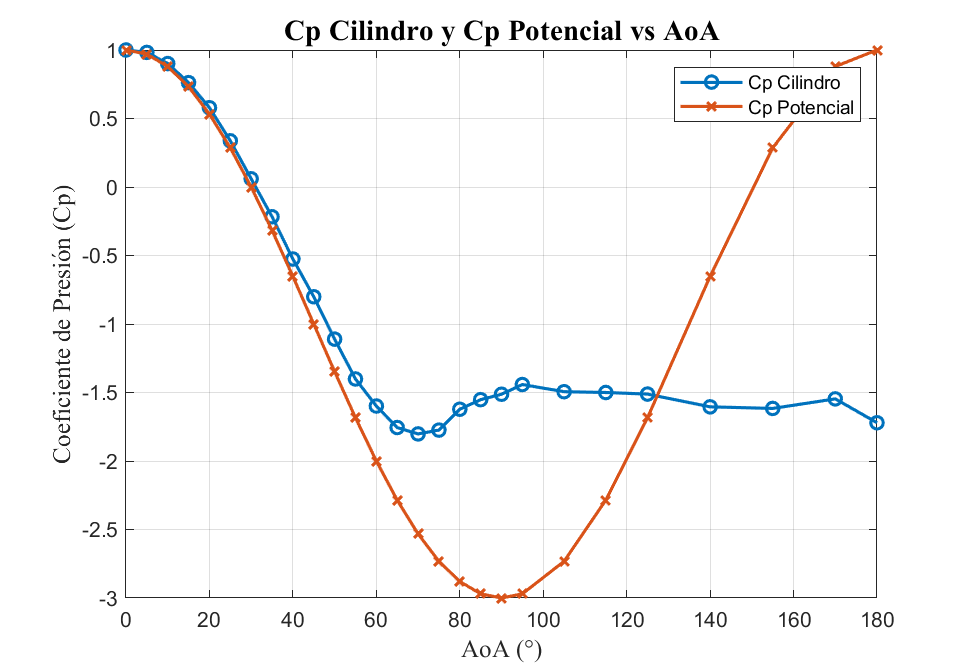
\includegraphics[width=0.9\textwidth]{01.Parte1/Figuras/Cilindro_Cp.png}
    \caption{Comparação entre o coeficiente de pressão do
experimento e o coeficiente de pressão potencial}
    \label{fig:Cp}
\end{figure}


\begin{figure}[htbp]
    \centering
    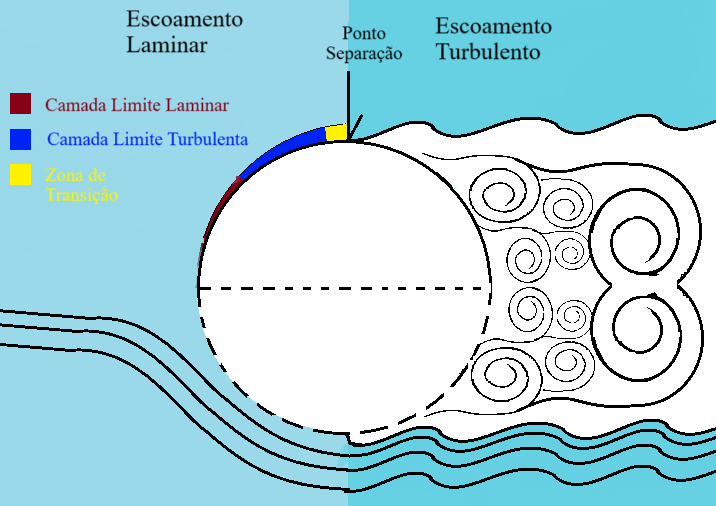
\includegraphics[width=0.9\textwidth]{01.Parte1/Figuras/Clindrof.png}
    \caption{Representação dos análises, adaptado de \cite{anderson2016introduction} - Figura 5.75, p. 402.}
    \label{fig:CilindroAnderson}
\end{figure}


\subsubsection{Desprendimiento de Fluxo}

 O fluxo é subsônico $ Mach = 0.05 \pm 1.9 \cdot 10^{-5} $. Como se evidencia, a separação do fluxo ocorre após os $88^\circ \pm 0.5^\circ$, um ponto onde o fluxo não consegue seguir a superfície do cilindro devido à queda de velocidade. Isso pode ser observado porque a inclinação da curva deixa de seguir o $C_P$ potencial e se torna aproximadamente constante.
\begin{equation}
   \frac{dC_{p}}{dAoA} = Cte ~~ ; ~~  C_P = -1.5 \pm 0.42
\end{equation}

% ----------------------------------------------------------------------

\subsubsection{Capa limite}
De $0^\circ \pm 0.5^\circ$ a $40^\circ \pm 0.5^\circ$ pode-se considerar laminar, uma vez que segue a linha de $C_P$ potencial (fluxo subsônico sem viscosidade), comparável a dizer que segue um fluxo que 'não possui fricção' na superfície. Experimentalmente, diz-se que é desprezível ao ter uma camada limite muito fina.


\begin{equation}
\begin{aligned}
\text{Laminar: } & \left| \frac{dC_{p}}{dAoA} - \frac{d\bar{C}_{p}}{dAoA_\infty} \right| = 0~~ ; ~~  -0.5 < C_P < 1\\ 
\text{Turbulento: } & \left| \frac{dC_{p}}{dAoA} - \frac{d\bar{C}_{p}}{dAoA_\infty} \right| > 0 ~~; ~~  -1.8 < C_P < -0.5 
\end{aligned}
\end{equation}


Depois de $40^\circ \pm 0.5^\circ$, temos uma transição para a camada limite turbulenta, pois a variação de $C_P$ é evidente. Geralmente, o fluxo turbulento tende a ser mais resistente ao desprendimento. Isso se deve ao fato de que, ao haver uma mistura mais eficaz de momento dentro da camada limite turbulenta, a influência da viscosidade do fluxo reduz sua velocidade (na superfície), levando a $C_P$ mais altos.

% -------------------------------------------------------------------------

\subsubsection{Transicion flujo Laminar a Turbulento}
A transição foi determinada a partir do ponto onde a velocidade do fluxo diminui abruptamente. O fluxo laminar apresenta uma queda mais suave na pressão à medida que o ângulo do cilindro aumenta.
    
\begin{equation}
   \text{Ponto Transição:}~  \frac{dC_{p}}{dAoA} = 0 ~~ ; ~~  C_P = -1.8 \pm 0.42
\end{equation}  


 Da Figura \ref{fig:Cp}, conclui-se que a transição ocorre aos $70^\circ \pm 0.5^\circ$. Para o caso deste experimento, considerou-se fluxo laminar para ângulos $<70^\circ$. Após a transição para fluxo turbulento, a mudança de $C_p$ é mais abrupta, embora se evidencie que o fluxo ainda consegue aderir à superfície do cilindro. A zona de fluxo turbulento está atrás do cilindro; isso se sabe ao concluir que o coeficiente de pressão atrás do cilindro $>100^\circ \pm 0.5^\circ$ se mantém constante, devido ao fato de que a velocidade do fluxo não muda.





% El desprendimiento de flujo ocurre en la región posterior del cilindro, donde el flujo no puede seguir la curvatura de la superficie debido a la caída de velocidad, lo que genera una zona de recirculación.

% El Cp se vuelve aproximadamente constante o deja de seguir la tendencia esperada a medida que el flujo se separa de la superficie. Este punto de desprendimiento suele estar alrededor de los 120°-150° medidos desde el frente (stagnation point) del cilindro.
% Transición de flujo laminar a turbulento:

% La transición ocurre antes del desprendimiento, cuando el flujo laminar se convierte en turbulento.
% En el gráfico de Cp, el flujo laminar muestra una caída más suave en la presión conforme se mueve desde la parte delantera hacia los costados del cilindro.
% Después de la transición a flujo turbulento, el descenso de Cp puede volverse más abrupto. Además, en la región de flujo turbulento, los valores de Cp pueden ser más bajos que en el flujo laminar, ya que el flujo turbulento puede adherirse más tiempo a la superficie del cilindro.